\documentclass{standalone}
\usepackage{tikz}
\usetikzlibrary{automata, positioning, arrows}

\begin{document}
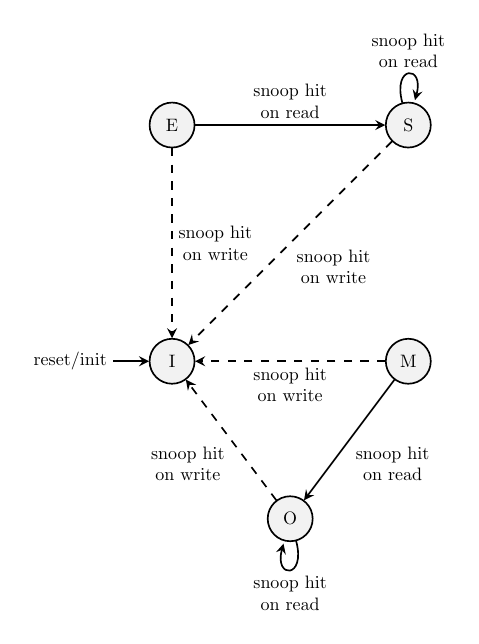
\begin{tikzpicture}[initial text={reset/init}]
\tikzstyle{every node}=[scale=0.65]
\tikzstyle{every state}=[semithick, fill=gray!10]
\tikzstyle{every edge}=[draw,->,>=stealth,auto,semithick]

\node[state] at (0,3) (E) {E};
\node[state] at (3,0) (M) {M};
\node[state, initial] at (0,0) (I) {I};
\node[state] at (3,3) (S) {S};
\node[state] at (1.5,-2) (O) {O};

\draw (M) edge[dashed] node[align=center] {snoop hit\\on write} (I)
        edge node[align=center] {snoop hit\\on read} (O);
\draw (S) edge[dashed] node[align=center] {snoop hit\\on write} (I)
        edge[loop above] node[align=center] {snoop hit\\on read} (S);
\draw (E) edge[dashed] node[align=center] {snoop hit\\on write} (I)
        edge node[align=center] {snoop hit\\on read} (S);
\draw (O) edge[loop below] node[align=center] {snoop hit\\on read} (O)
        edge[dashed] node[align=center] {snoop hit\\on write} (I);
\end{tikzpicture}
\end{document}
